\chapter{Dynamic Models: Part 2}\label{c:model2}
So far we have examined two mathematical models to predict and quantify the response of mechanical systems: a static (zero-order) model and a first-order dynamic model.  It may not be terribly surprising that our next topic is a second-order model.  A second-order model is a generic mathematical description of a system that is capable of oscillations. (You might recall that neither a static response nor a first-order response oscillates.)   This simple model can be used to help understand the behavior of a variety of engineering systems such as
\begin{itemize}
\item pendulums, where the position oscillates
\item passive circuits, where the voltage/current oscillates 
\item acoustic systems, where the sound pressure level (volume) oscillates.
\end{itemize}

The key elements of a second-order model are \emph{inertia}, \emph{stiffness} and \emph{damping} where the interpretation of these elements depends on the domain (mechanical, electrical, acoustic, etc.) under examination.  We will focus on mechanical systems where the inertia is in the form of mass, the stiffness is a restoring force (such as a spring or gravity) and damping is losses due to frictional forces.

\input{MModel2_secondorder.tex}

\input{MModel2_exbeam.tex}

\section{Measuring Second-Order Response}
For physical systems that exhibit oscillatory response we can ``fit'' a second-order response to the system measurements to estimate the system parameters ($\omega_n$ and $\zeta$) based on the measured response.  In other words, consider that you measure the time response of a system (e.g., a cantilevered beam, a RLC circuit, etc.) and you observe that the behavior looks something like Figure~\ref{f:secondfreeresp}.  How can you estimate the natural frequency and damping ratio associated with such a response?

\begin{figure}[h!bt]
\centerline{
{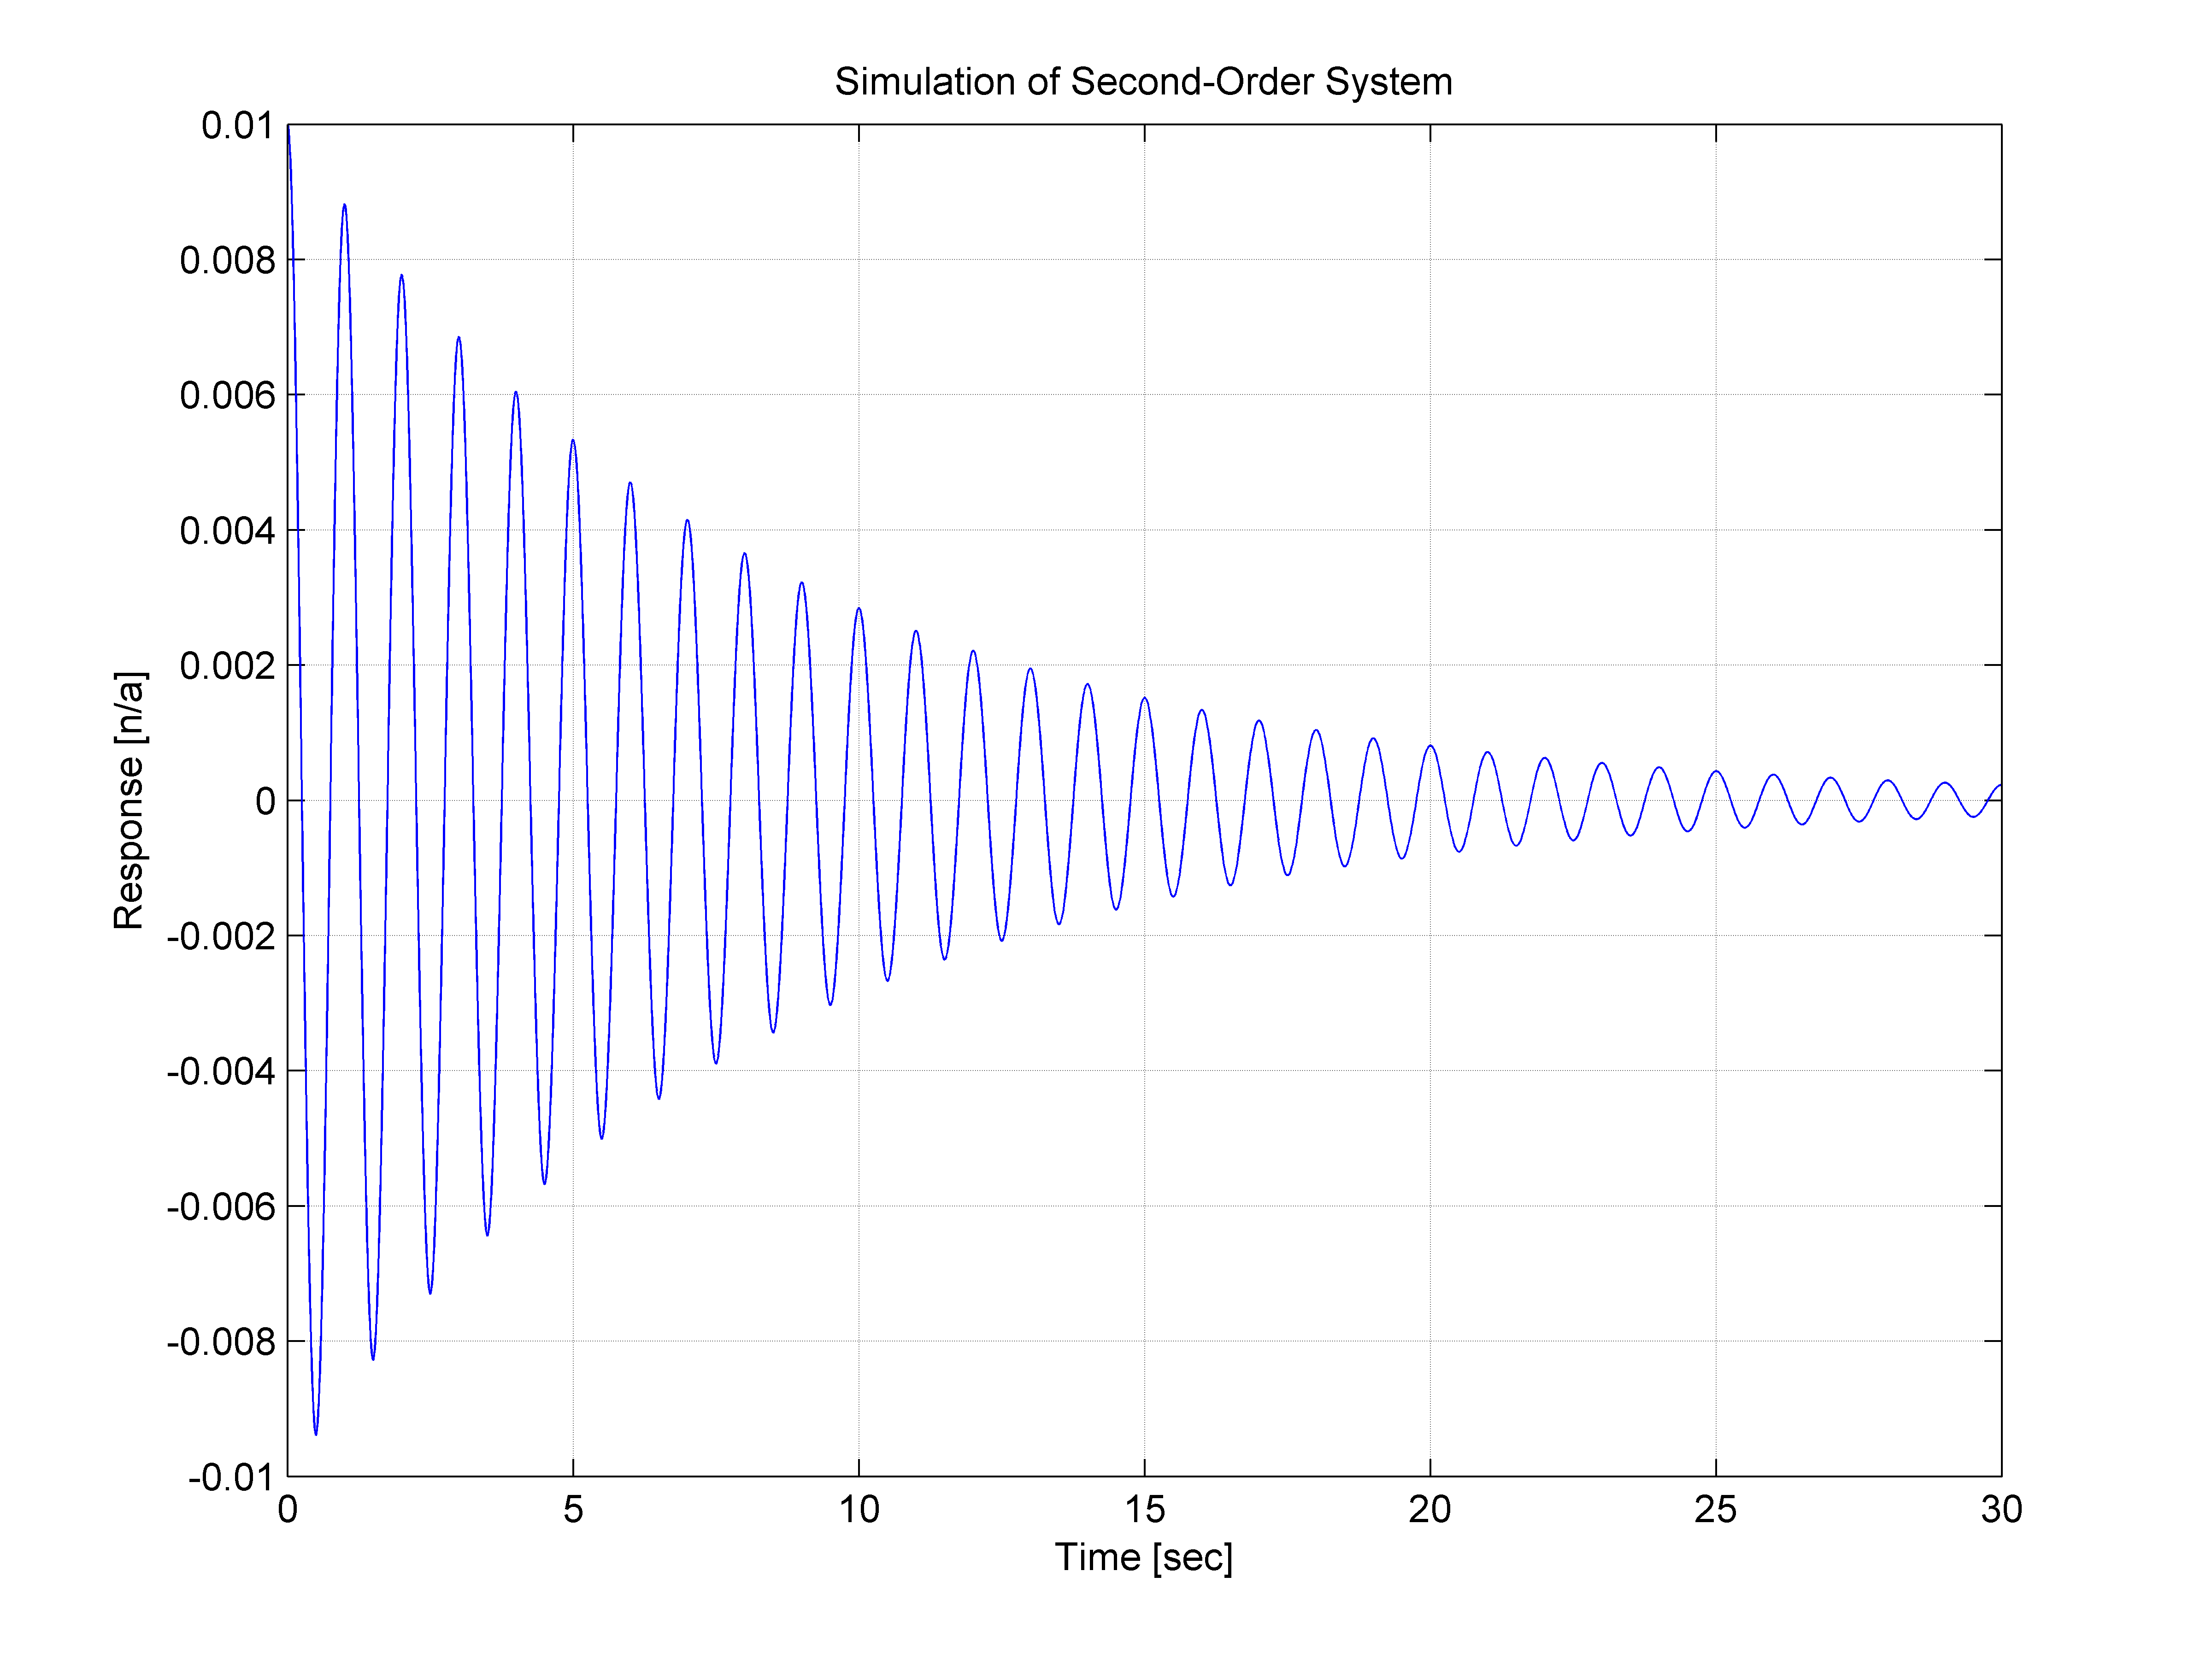
\includegraphics[width=0.6\textwidth]{second_order_grid.png}}}
\caption{Illustration of the free-response of a second-order system.  The response shows the analytical solution for $y(t)$.}
\label{f:secondfreeresp}
\end{figure}

\subsection{Measuring Frequency}
It may be obvious, but if for no other reason than to get the units (\unit[]{Hz} and \unitfrac[]{rad}{s}) it is worth spending a little time discussing how to measure the frequency of oscillation from a measured response.  Since our measurements are of the {\bf time} response, we will need to start by estimating the period of oscillation, the time it takes for one cycle of oscillation.  We could do this by measuring the time between two adjacent peaks in the response, but a better way is to measure the elapsed time ($\Delta t$) between two peaks (or troughs, or zero-crossings) of the response and the number of cycles ($n$) as illustrated in Figure~\ref{f:secondtime}.
\begin{figure}[h!bt]
\centerline{
{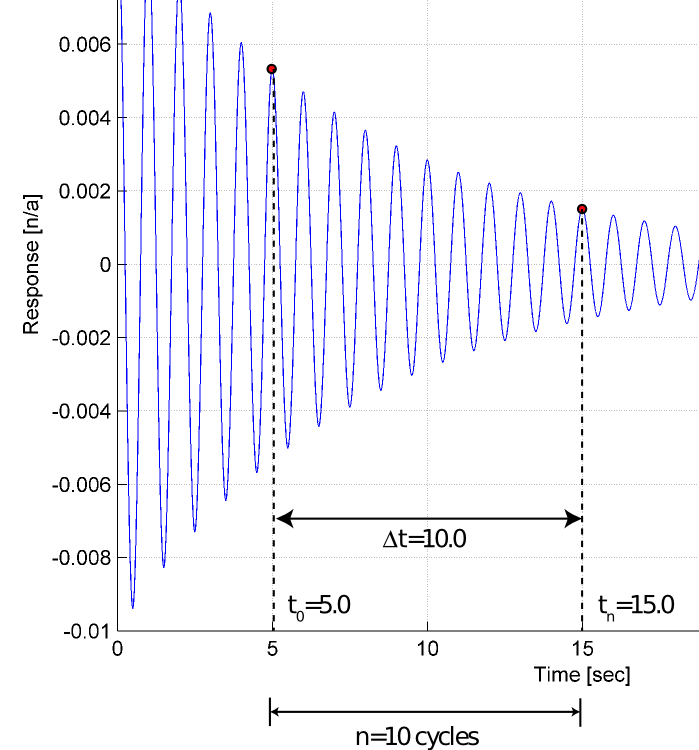
\includegraphics[width=0.6\textwidth]{second_order_grid_time_only_annote_crop.png}}}
\caption{Illustration of measuring the period of oscillation.}
\label{f:secondtime}
\end{figure}
Then we can estimate the average period of oscillation as
\begin{equation}
T = \frac{t_n-t_o}{n}=\frac{\Delta t}{n}=\frac{\unit[10.0]{s}}{\unit[10]{cycles}} = \unitfrac[1.0]{s}{cycle}.
\end{equation}
The corresponding frequency of oscillation ($f_d$ (in Hz)) is the reciprocal of the period
\begin{equation}
f_d = \frac{1}{T} = \frac{1}{\unitfrac[1.0]{s}{cycle}} = \unitfrac[1.0]{cycles}{s} = \unit[1.0]{Hz}.
\end{equation}
The last step is to convert the units of this frequency from Hz to \unitfrac[]{rad}{s} with the expression
\begin{equation}
\omega_d = f_d (2 \pi) = \unitfrac[1.0]{cycles}{s} (\unitfrac[2 \pi]{rad}{cycle}) = \unitfrac[6.28]{rad}{s}.
\end{equation}
It is important to notice that what we have estimated here is the {\bf damped} natural frequency ($\omega_d$), not the undamped natural frequency ($\omega_n$).  Again, the relationship between these two quantities is
\begin{equation}
\omega_n = \frac{\omega_d}{\sqrt{1-\zeta^2}}.
\end{equation}
To estimate $\omega_n$ we'll need to know (to estimate) the damping ratio ($\zeta$).

\subsection{Measuring the Damping Ratio Via Logarithmic Decrement Method}

The logarithmic decrement method is a technique to empirically identify the damping ratio ($\zeta$) of a second-order underdamped model.  The method is based on the characteristic time response of the model.  The time response can be either the response to a step input or the free-response to a non-zero initial condition.  The free-response to an initial condition is given in your textbook as
\begin{equation}
y_h(t)=C e^{-\zeta\omega_nt}\sin\left(\omega_dt+\phi\right) 
\end{equation}
where $\omega_n$ is the undamped natural frequency of the system and $\omega_d=\omega_n\sqrt{1-\zeta^2}$ is the damped natural frequency.  The two constants $C$ and $\phi$ are determined from the initial conditions.

To estimate the damping ratio can be estimated in the following way.  First plot the response $y(t)$ as a function of time.  Choose two peaks of the oscillatory response $y_0$ and $y_n$ where $y_0$ is the larger value that happens earlier in time.  Calculate the logarithmic decrement ($\delta$) as
\[ \delta = \frac{1}{n}\ln\left(\frac{y_0}{y_n}\right) \]
where $n$ is the number of cycles between $y_0$ and $y_n$.
Finally calculate the damping ratio as
\[ \zeta = \frac{1}{\sqrt{1+\left(\frac{2\pi}{\delta}\right)^2}}. \]

\subsubsection{Example}
Figure \ref{f:secondfreeresp} illustrates the free response of a second-order model to an initial condition of $y(0)=0.01$ and $\dot{y}(0)=0$.  The undamped natural frequency is \unitfrac[$2 \pi$]{rad}{s}.

To calculate the logarithmic decrement we need to select two peaks from the response as shown in Figure~\ref{f:resp2}\footnote{The MATLAB function \texttt{ginput()} is handy for selecting the values from a figure window.}. These selected values, along with the equations above, result in $\delta=0.124$ and $\zeta=0.0198$.  This estimate is quite close to the value of 0.02 which was used to generate the example.

\begin{figure}[h!bt]
\centerline{
{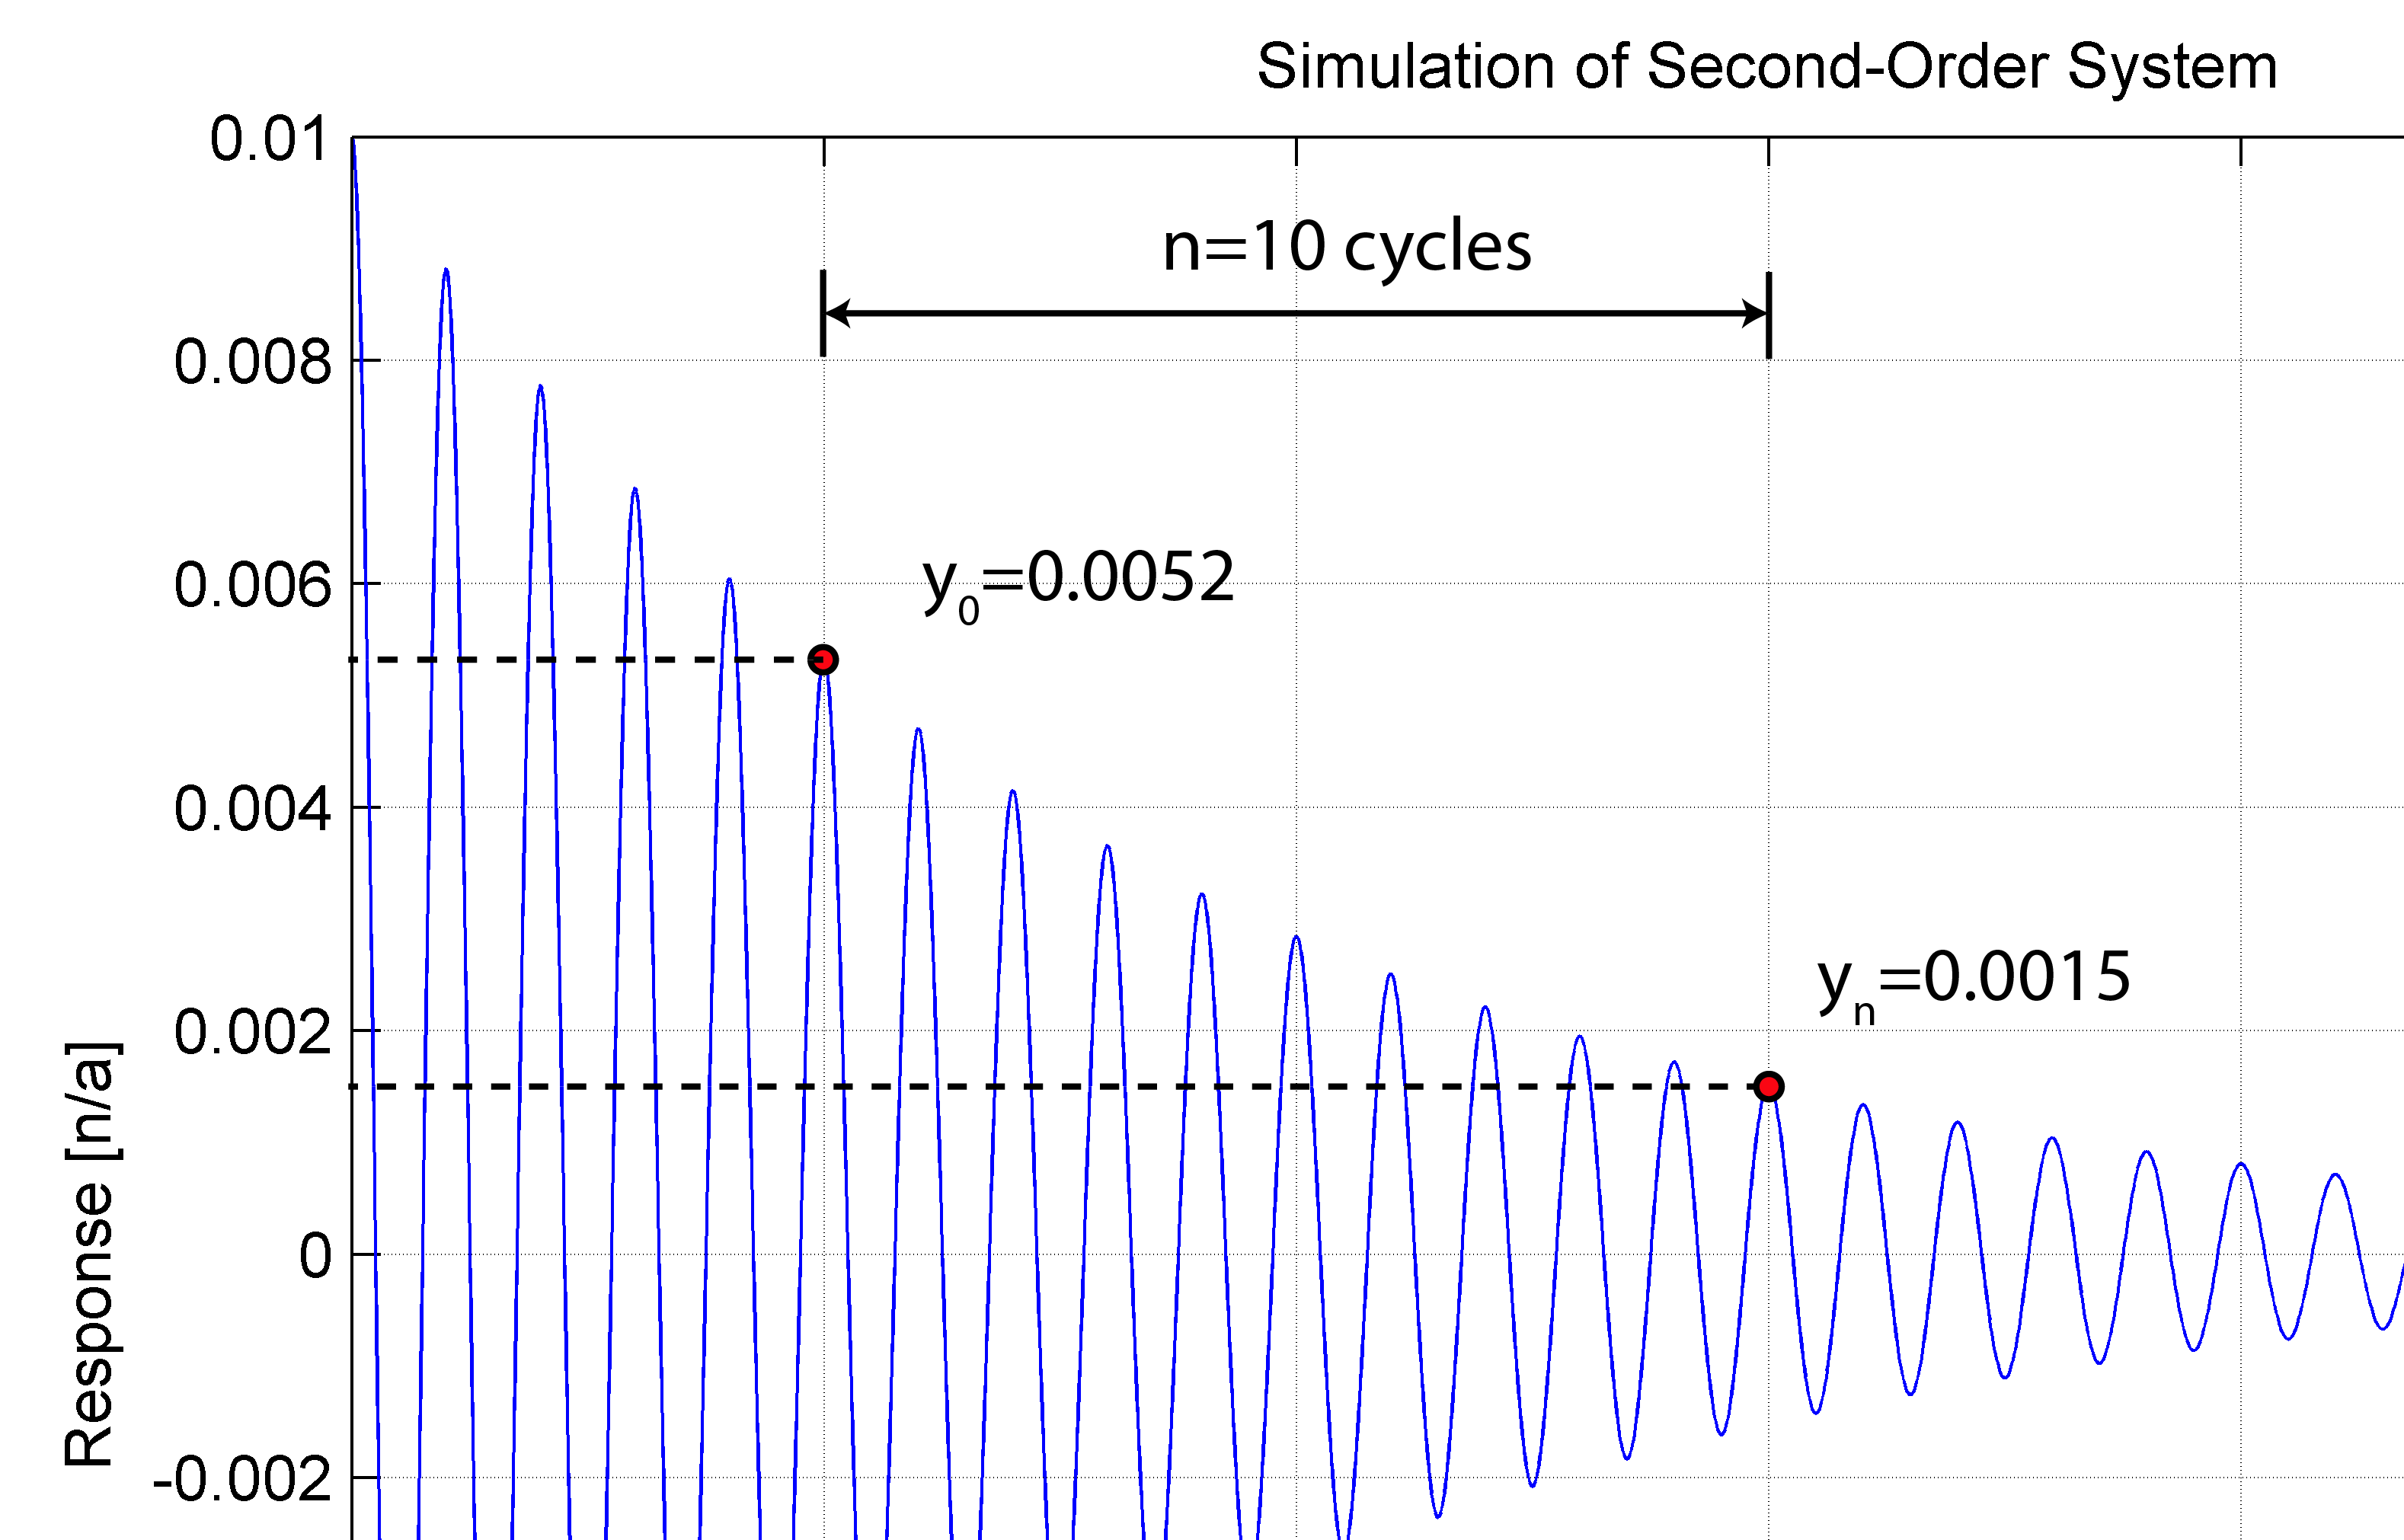
\includegraphics[width=0.6\textwidth]{second_order_grid_annote_crop.png}}}
\caption{The added annotation illustrates the selection of ``peaks'' in the response to initiate the logarithmic decrement process.}
\label{f:resp2}
\end{figure}

%\afterpage{\clearpage}

\subsubsection{Why It Works}
The logarithmic decrement method is based on fitting a curve to the data.  In this case the curve (the model) is the exponential amplitude of the second-order response
\begin{equation}
y_{env}(t)=C e^{-\zeta\omega_nt}.
\label{e:env}
\end{equation}
This function is superimposed on the response in Figure~\ref{f:env}.
\begin{figure}[h!bt]
\centerline{
{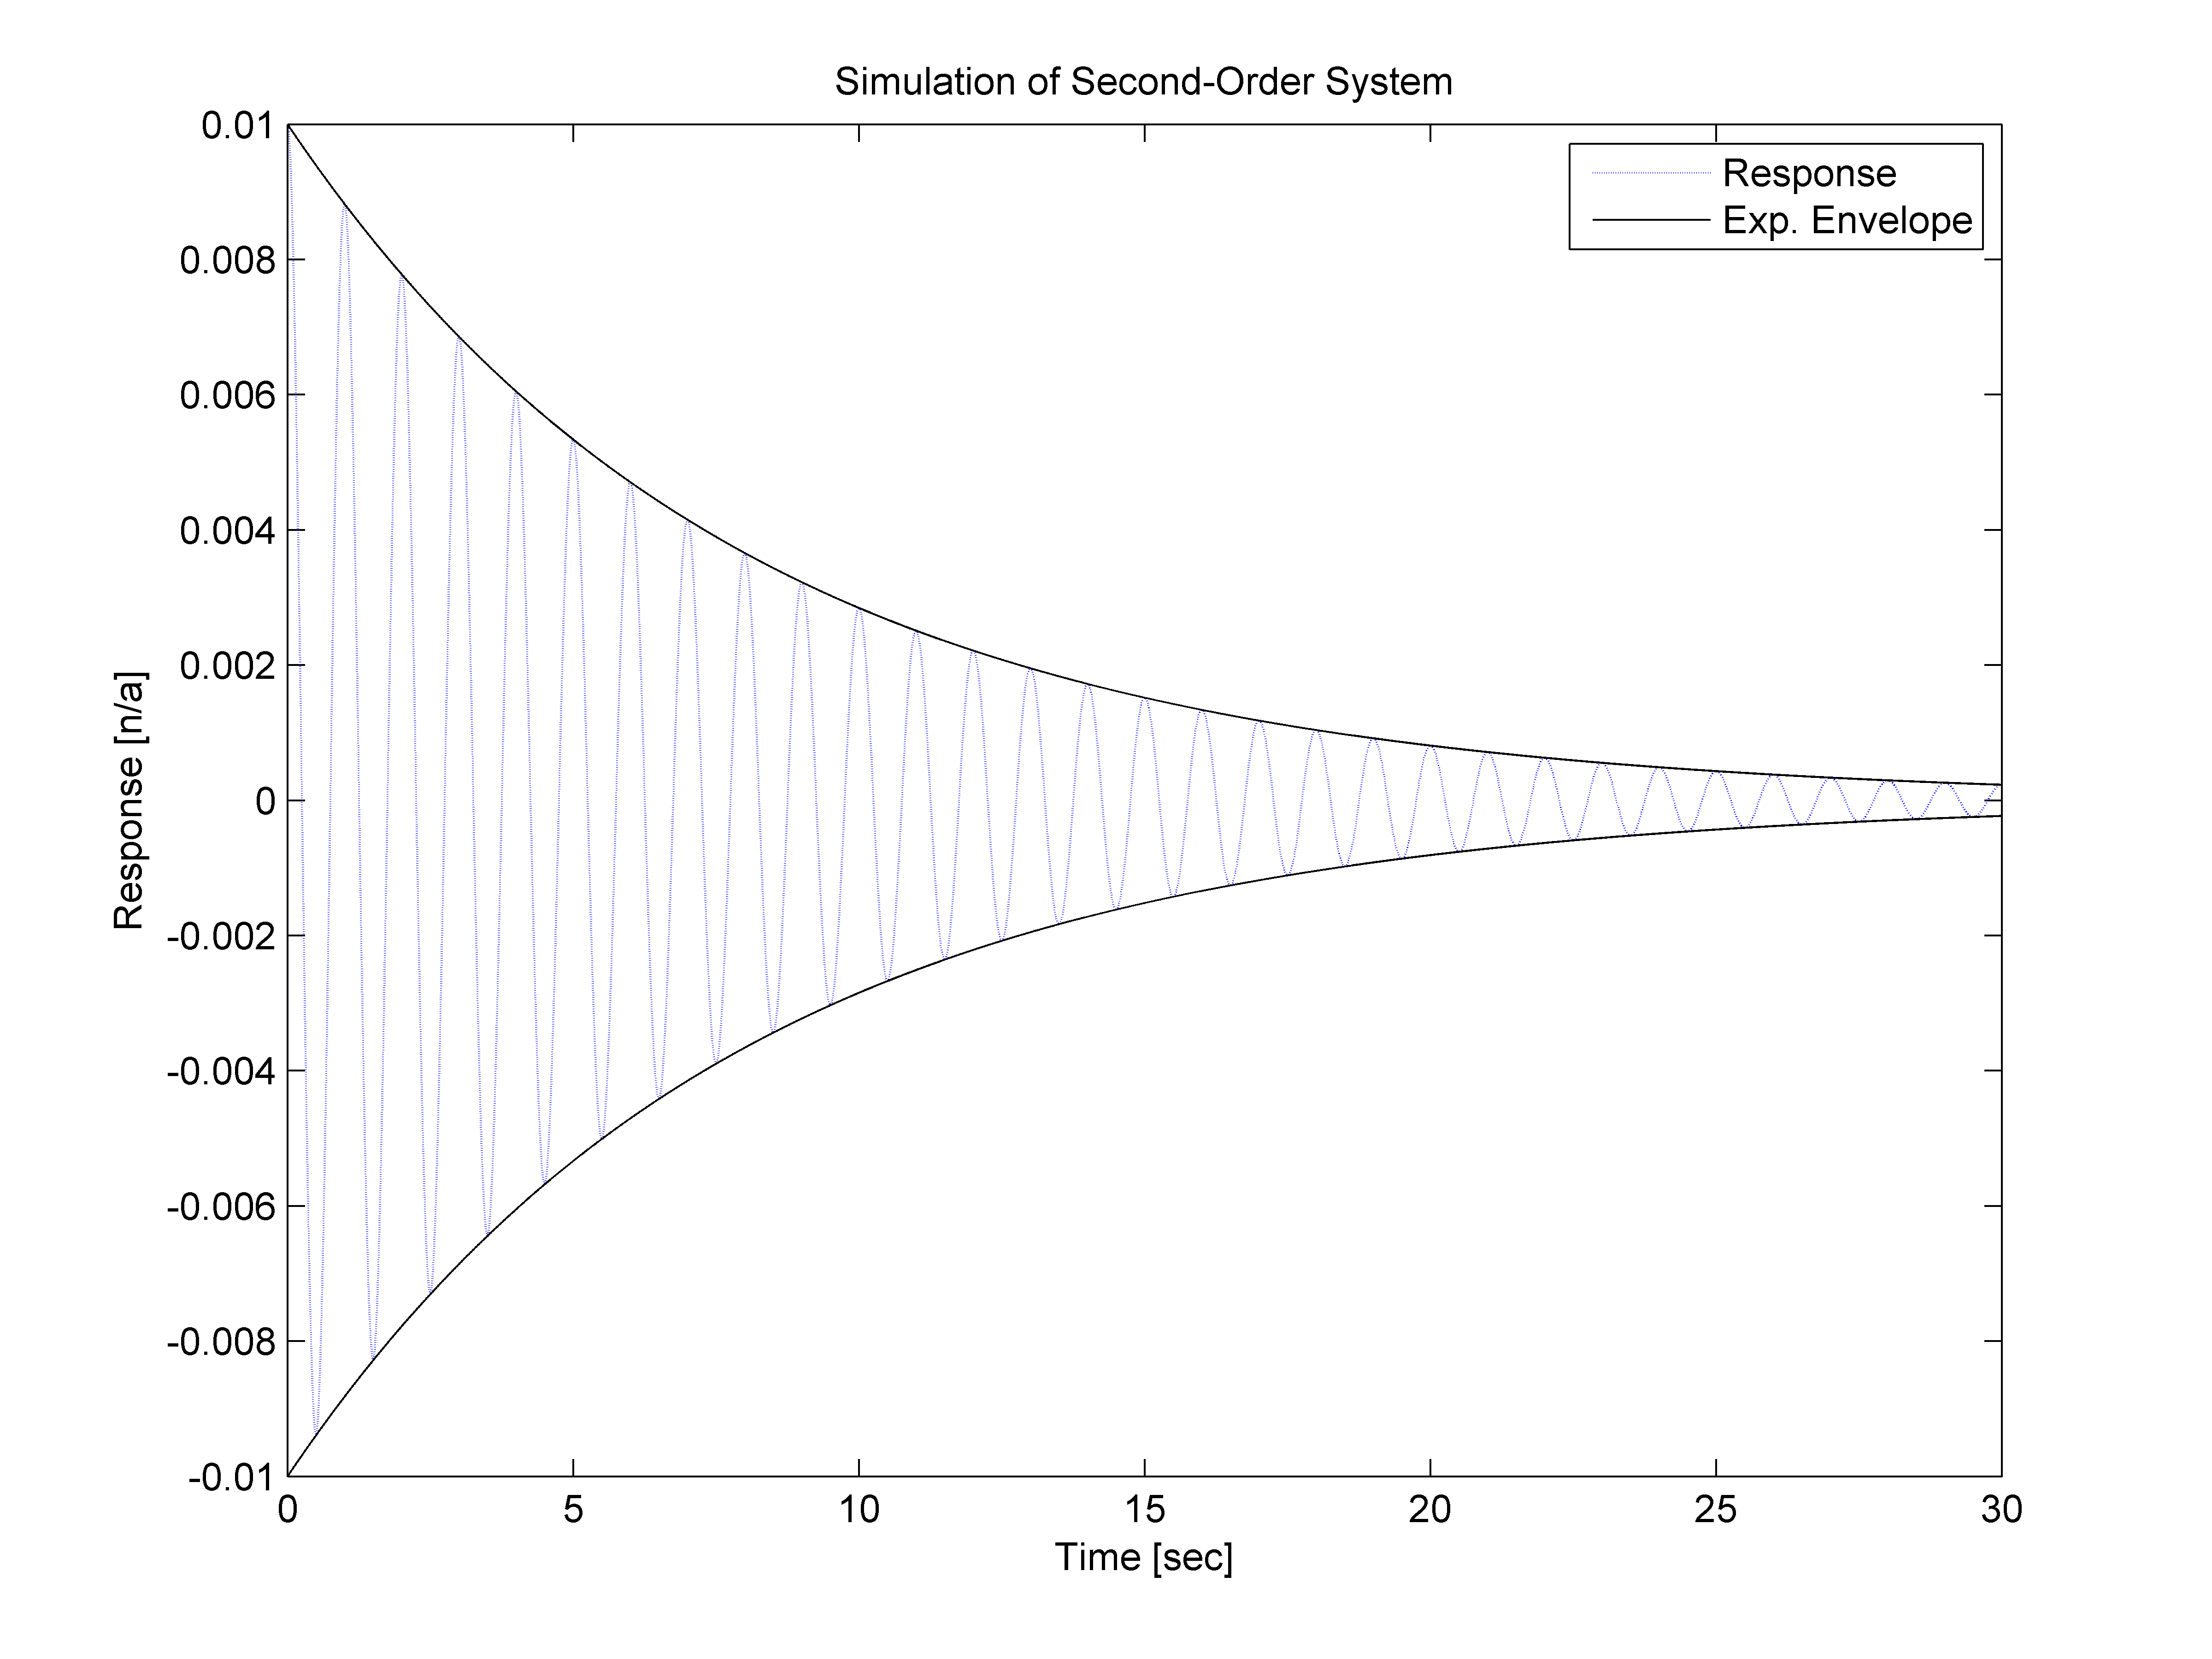
\includegraphics[width=0.6\textwidth]{second_order_env.png}}}
\caption{Second-order free response with the exponential envelope function included (\ref{e:env})}.
\label{f:env}
\end{figure}

If we take the natural logarithm of this function we get a linear relationship between $Y_{ln}=\ln(y_{env})$ and $t$:
\[
Y_{ln}=\ln(y_{env})=(-\zeta \omega_n) t.
\]
This linear relationship is illustrated in Figure~\ref{f:ln} where $Y_{ln}$ is plotted versus time.  The slope of the line is $m=-\zeta \omega_n$.
\begin{figure}[hbt!]
\centerline{
{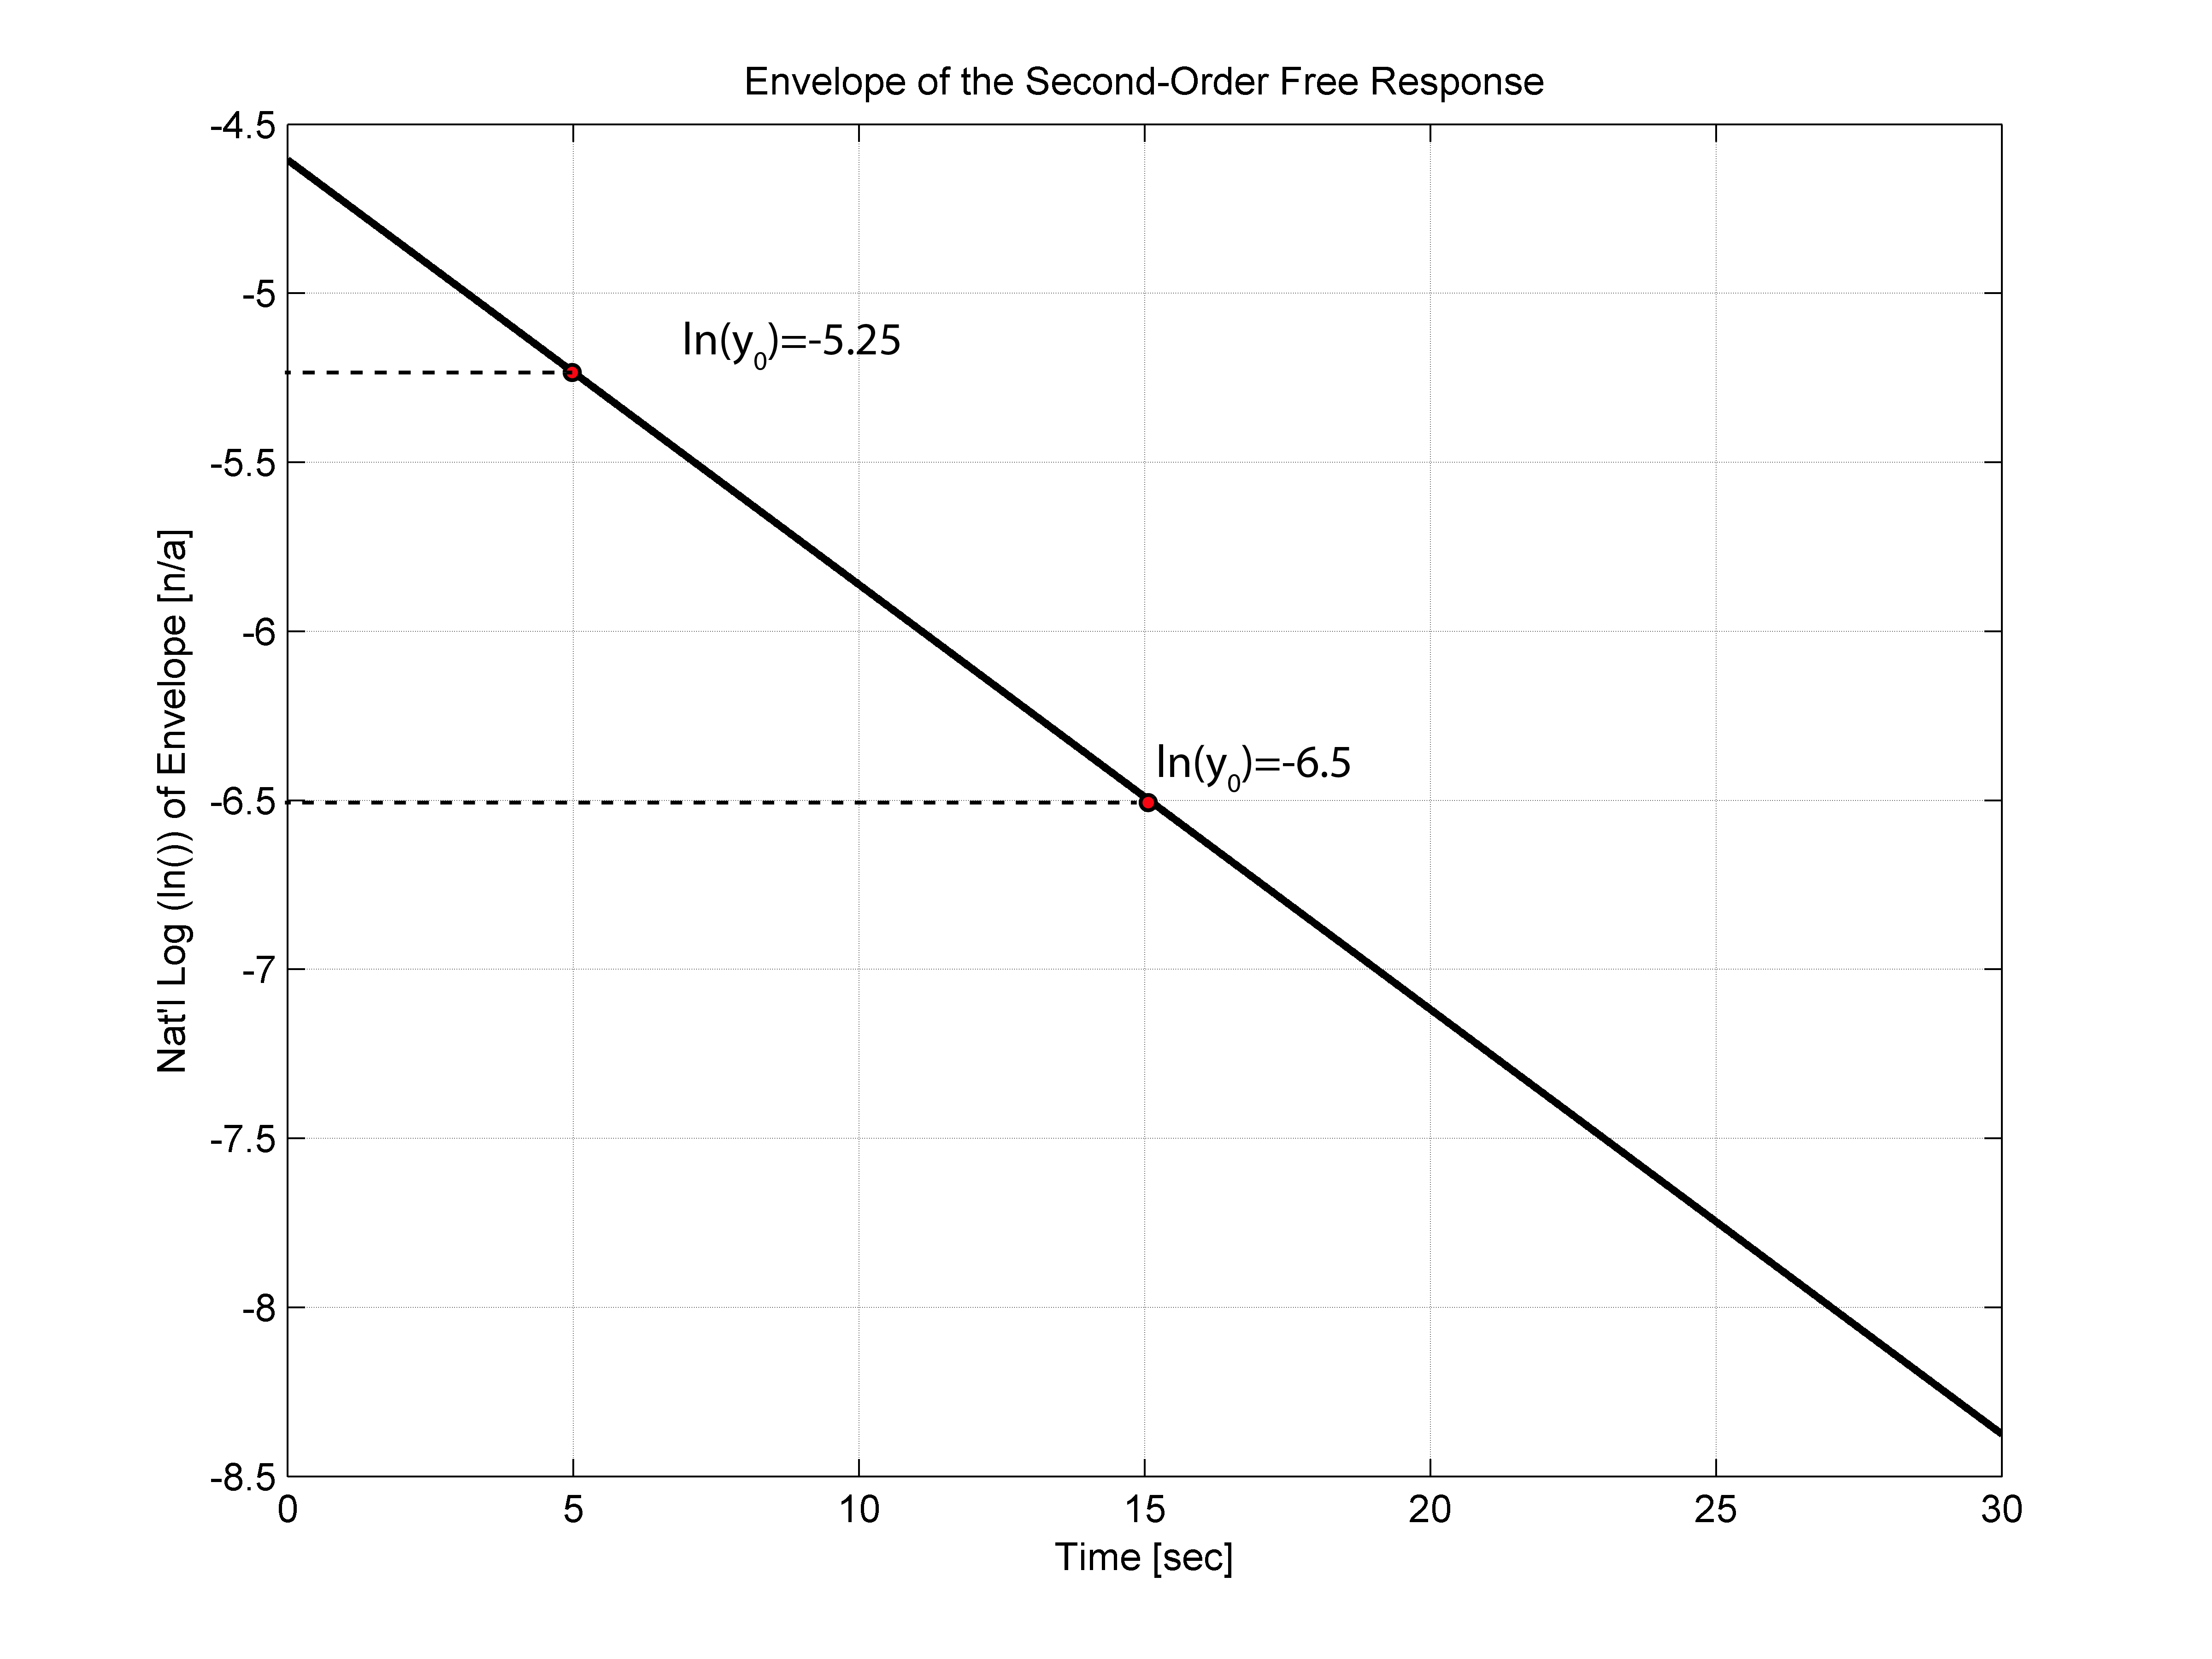
\includegraphics[width=0.6\textwidth]{second_order_env_ln_annote.png}}}
\caption{Plot of the exponential envelope shown in Figure~\ref{f:env}, but here the natural logarithm ($\ln()$) of the amplitude is plotted, i.e., $Y_{ln}$.}
\label{f:ln}
\end{figure}

Because we are using the second-order response model, we now just need to find the slope of the line in Figure~\ref{f:ln} and solve for the damping ratio.  The slope of the line can be expressed as
\begin{eqnarray}
m & = & \frac{\ln(y_0)-\ln(y_n)}{t_0-t_n}=-\zeta \omega_n \\
\label{e:slope} \\
m & = & \frac{\ln(y_0)-\ln(y_n)}{t_n-t_0}=\zeta \omega_n. \\
\label{e:slope2}
\end{eqnarray}
We can use (\ref{e:slope}) or (\ref{e:slope2} directly, but we have to deal with the fact that we don't know $\omega_n$.  It is important to note that the frequency of oscillation is the damped natural frequency ($\omega_d$) which is related to the undamped natural frequency by the relationship
\begin{equation}
\omega_d=\omega_n\sqrt{1-\zeta^2}.
\label{e:omegas}
\end{equation}
The logarithmic decrement method uses the peaks of the oscillating response to get around this trouble.  We know that the change in time is an integer number of periods of oscillation at the damped natural frequency
\begin{equation}
t_n-t_0 = \frac{n}{\omega_d / 2 \pi}.
\label{e:time}
\end{equation}
Now we can substitute (\ref{e:time}) and (\ref{e:omegas}) into (\ref{e:slope2}) to get
\[
\frac{\ln\left(\frac{y_0}{y_n}\right)}{n (2 \pi)} \omega_d = \zeta \omega_n
\]
and
\[
\frac{\ln\left(\frac{y_0}{y_n}\right)}{n (2 \pi)} \omega_n \sqrt{1-\zeta^2} = \zeta \omega_n.
\]
Next, let 
\[ \delta = \frac{1}{n}\ln\left(\frac{y_0}{y_n}\right) \]
and we solve for $\zeta$
\[
\zeta^2=\frac{\left(\frac{\delta}{2 \pi}\right)^2}{1+\left(\frac{\delta}{2 \pi}\right)^2}
\]
\[ \zeta = \frac{1}{\sqrt{1+\left(\frac{2\pi}{\delta}\right)^2}}. \]

It is interesting to consider that the logarithmic decrement method is doing this linear-fit with just two data points.  It would be interesting to do this linear fit with multiple data points using a least-squares approach to identify the damping ratio.  One advantage (along with a more precise result) is that you would be able to quantify the ``goodness-of-fit'' for the data using the correlation coefficient ($R^2$).




